\section{Prompts}
\label{app:prompts}
The prompts are verbatim from the code that produced the results. The examples use placeholder passages; in the runs every condition except removal shows the generator the same passages (checked against the run records).
\paragraph{Generation skeleton.}
\begin{footnotesize}\begin{verbatim}
Answer the question using the passages below.
If the passages support more than one valid answer
(for example, different people or things share the
same name), give every valid answer.
If no passage answers the question, the answer is
"unknown".
{instruction}
{context}
{conflicts}
Question: {question}

Give a brief explanation, then end with one line in
exactly this format:
Final answer(s): <answer 1> | <answer 2> | ...
\end{verbatim}\end{footnotesize}
\paragraph{Instruction v1.}
\begin{footnotesize}\begin{verbatim}
Some passages may contradict each other. Before
answering, check whether they do.
Ignore passages that appear to contain
misinformation, and if a disagreement reflects
genuinely different valid answers, report each one.
\end{verbatim}\end{footnotesize}
\paragraph{Instruction v2.}
\begin{footnotesize}\begin{verbatim}
Some passages may contain false information. Before
answering, decide which passages are reliable by
checking them against each other.
Do not include an answer that is supported only by a
passage you judge to be unreliable.
\end{verbatim}\end{footnotesize}
\paragraph{Example: directional flag (passage 2 suspect).}
\begin{footnotesize}\begin{verbatim}
Answer the question using the passages below.
If the passages support more than one valid answer
(for example, different people or things share the
same name), give every valid answer.
If no passage answers the question, the answer is
"unknown".

Passage 0 [POTENTIAL CONFLICT with passage(s): 2]:
<passage 0>

Passage 1:
<passage 1>

Passage 2 [LIKELY MISINFORMATION; conflicts with
passage(s): 0]:
<passage 2>

POTENTIAL CONFLICTS DETECTED:
- Passages 0 and 2: possible contradiction; passage
2 likely contains misinformation

Question: Who founded X?

Give a brief explanation, then end with one line in
exactly this format:
Final answer(s): <answer 1> | <answer 2> | ...
\end{verbatim}\end{footnotesize}
\paragraph{Directional LLM detector.}
\begin{footnotesize}\begin{verbatim}
You will see a question and {n} numbered passages
retrieved for it.
Some passages may contain misinformation: false
claims about the answer to the question.
Identify every pair of passages that CONTRADICT each
other about the answer to the question,
i.e. they cannot both be true about the same entity
at the same time. Passages that are about
different entities with the same name, give
complementary details, or describe different times
are NOT contradictions; note them as "ambiguity",
"complementary" or "temporal" instead.

For each contradiction, say which passage of the
pair is more likely the misinformation, judging
by agreement with the other passages and by
plausibility: its number, "both" if both are likely
false, or "unclear" if you cannot tell.

Question: {question}

{passages}

Return JSON only: {{"pairs": [{{"i": <int>, "j":
<int>, "relation":
"contradiction|ambiguity|complementary|temporal",
"misinformation": <int>|"both"|"unclear"}}]}}
Use the passage numbers shown. "misinformation" is
needed only for contradictions. Return {{"pairs":
[]}} if there are none.
\end{verbatim}\end{footnotesize}


\section{Additional Results}
\label{app:extra}

\paragraph{Published baselines (H14).} Astute RAG \citep{wang2025astute} and TrustRAG \citep{zhou2025trustrag} lose same-name answers
on RAMDocs (H14). On ConflictBank, the registered H14 compared our pipeline's multi-answer prompt with the
baselines' own one-answer prompts. Under the matched one-answer prompt (our principal comparison), our pipeline beats them by
\hFourteenMatchedAst\ and \hFourteenMatchedTr\ points (exploratory). Our TrustRAG port
first omitted the repository's system message; sending it (\S17.2) changes TrustRAG's accuracy by \blTrustSysCb\
points on ConflictBank, \blTrustSysMj\ under majority misinformation and \blTrustSysRd\ on RAMDocs (\blTrustSysRdMulti\
for its multi-answer variant). Against the corrected TrustRAG, with policies matched (Holm over the four), the LLM
directional flag changes accuracy by \blHFourteenCbs\ on ConflictBank (one-answer), \blHFourteenRd\ on RAMDocs (multi-answer),
\blHFourteenMj\ under majority misinformation, and \blHFourteenCb\ under the registered mismatched prompts.
On ConflictBank, NLI first saw passage prefixes that usually omit the changed fact. Cutting each passage to the
sentences closest to the question, up to the registered 1,500 characters, keeps both answers, but the
pair still exceeds the cross-encoder's 512 tokens and NLI flags no pair (pair recall \detNliWinRecall\%). With
300 characters, about one sentence (a disclosed deviation, \S17.6), NLI finds \detNliSentRecall\% of the gold pairs at
\detNliSentPrec\% pair precision and flags \detNliSentCleanFpr\% of clean questions. Its flag changes conflict
accuracy by \blNliSentFlag\ points (removal: \blNliSentRem). A single call that names suspect passages before
answering does not differ significantly from the pipeline (H18; Table~\ref{tab:baselines}).

\paragraph{Robustness to the metric and the labels.}
Table~\ref{tab:main_robust} repeats Table~\ref{tab:main} with the bidirectional metric, and Table~\ref{tab:contains}
repeats the pre-registered tests treating every suspect document as misinformation. Table~\ref{tab:hypotheses}
lists all pre-registered tests.

\begin{table*}[t]
\centering\footnotesize
\setlength{\tabcolsep}{4pt}
\begin{tabular}{p{7.4cm}p{3.6cm}p{4.2cm}}
\toprule
Claim (section) & Evidence & Status \\
\midrule
A correct neutral flag lowers RAMDocs accuracy (\S\ref{sec:neutral}) & H2, H9 & registered before any confirmatory data \\
Its mechanism depends on the answer policy: added misinformation, abstention, little effect (\S\ref{sec:neutral}) & Table~\ref{tab:risk}; H15, H19--H21, H25, H26 & answer mix: re-analysis; tests: registered addenda \\
Pooled effect, policy split, moderators, utility, transitions (\S\ref{sec:neutral}) & Tables~\ref{tab:pooled}, \ref{tab:utility} & re-analysis of data already seen; dependence: \S17 \\
The directional flag beats the neutral one (\S\ref{sec:direction}) & H3, H9--H12, H15, H16, H19, H25, H26 & H3: before any confirmatory data; rest: addenda \\
Oracle direction is close to an answer key (\S\ref{sec:direction}) & H23 and its TOST & registered addendum; TOST registered in \S13.4 \\
Pooled, oracle direction is equivalent to an answer key on average, under the matcher (\S\ref{sec:direction}) & pooled H23; per-comparison TOST & unregistered re-analysis; heterogeneity: \S17 \\
Under the judge, neither pooled equivalence holds (\S\ref{sec:direction}, \S\ref{sec:real}) & H38 & registered (\S19), LLM judge \\
Direction helps and a neutral flag does not on real web pages (\S\ref{sec:direction}) & H37 & registered (\S19); labels as released \\
Real-detector gains depend on the generator (\S\ref{sec:real}) & H15, H17, H19, H25, H26 & registered addenda \\
Right flags gain less than wrong flags cost; similar follow rates (\S\ref{sec:real}) & H31 & registered addendum (\S16) \\
Break-even direction precision rises with generator accuracy (\S\ref{sec:real}) & Table~\ref{tab:breakeven} & unregistered re-analysis \\
Break-even is a calibration, not a rule for selective detectors (\S\ref{sec:real}) & Table~\ref{tab:selection} & re-analysis (\S17) \\
Follow rates and coverage account for the crossed cells (\S\ref{sec:real}) & Figure~\ref{fig:reliability} & unregistered; retrospective \\
Frozen, the account predicts unseen ConflictBank cells; it overstates harm on clean questions and HealthContradict (\S\ref{sec:real}) & H32--H36, Table~\ref{tab:fresh} & registered (\S19), predictions committed first \\
Registered reliability gap correlates with the gain (\S\ref{sec:real}) & H24 & registered addendum (\S13), 5 of 30 cells existed \\
The gap is dominated by generator accuracy; precision and recall matter within generators (\S\ref{sec:real}) & Table~\ref{tab:h24redo} & re-analysis of data already seen \\
The detector's verdict as an answer key matches the flag; its model's answer as a hint does not (\S\ref{sec:real}) & H30, H27 & registered addenda (\S15, \S16); pooled TOST unregistered \\
A real detector's flag hurts when conflicts are rare (\S\ref{sec:real}) & Table~\ref{tab:prevalence} & unregistered re-analysis \\
Direction survives reordering and paraphrase (\S\ref{sec:real}) & H29 & registered addendum; equivalence not shown \\
Direction and removal harm genuine conflicts (\S\ref{sec:real}) & H28 & registered addendum \\
The matcher's errors do not overturn the directional conclusions (App.~\ref{app:semantic}) & Table~\ref{tab:semantic} & registered re-score (\S17), LLM judge \\
Recommendations (\S\ref{sec:discussion}) & -- & not tested end to end \\
\bottomrule
\end{tabular}
\caption{Status of each claim. \emph{Registered addendum}: committed before the runs it covers but
after earlier results were known. \emph{Re-analysis}: registered after the data were seen, or exploratory. The commit
history is the only timestamp.}
\label{tab:claims}
\end{table*}

\begin{table}[t]
\centering\small
\setlength{\tabcolsep}{4pt}
\begin{tabular}{@{}>{\raggedright\arraybackslash}p{3.3cm}rr@{}}
\toprule
Inverted oracle (names the correct side) & Conflict & Clean \\
\midrule
RAMDocs, directional flag & \advDirConf\ \advDirConfCI & \advDirClean \\
RAMDocs, removal & \advRemConf\ \advRemConfCI & \advRemClean \\
ConflictBank (multi-answer), directional flag & \zCbMiniOracleInvFlagDirectionalConflict & \zCbMiniOracleInvFlagDirectionalClean \\
\bottomrule
\end{tabular}
\caption{Adversarial control, gpt-4o-mini: change from no flags, in points (exploratory; \S9.5). On clean
questions the inverted oracle flags nothing (prompt unchanged).}
\label{tab:inverted}
\end{table}
\begin{table*}[t]
\centering\small
\setlength{\tabcolsep}{3.6pt}
\resizebox{\textwidth}{!}{%
\begin{tabular}{llrrrrrrrrrrr}
\toprule
& & & \multicolumn{2}{c}{Accuracy} & \multicolumn{4}{c}{Oracle pairs} & \multicolumn{2}{c}{LLM detector} & Single & LLM dir. \\
\cmidrule(lr){4-5}\cmidrule(lr){6-9}\cmidrule(lr){10-11}
Generator & Prompt & Seeds & Closed & Plain & Flag & One wrong & Dir.\ flag & Remove & Flag & Dir.\ flag & call & clean q. \\
\midrule
gpt-4o-mini & single & 3 & 10.0 & 51.1 & \textbf{$-$18.7} & \textbf{$-$35.7} & \textbf{$+$30.1} & \textbf{$+$35.0} & \textbf{$-$18.2} & $+$8.4 & $+$7.6 & $-$4.7 \\
gpt-4o-mini & multi & 3 & -- & 21.6 & \textbf{$-$8.8} & -- & \textbf{$+$27.9} & \textbf{$+$66.4} & \textbf{$-$8.4} & \textbf{$+$20.0} & -- & $-$1.0 \\
gpt-4o-mini & minimal & 3 & -- & 35.0 & \textbf{$-$18.1} & -- & \textbf{$+$38.4} & \textbf{$+$51.2} & -- & -- & -- & -- \\
gpt-4.1 & single & 1 & 20.0 & 64.7 & \textbf{$-$8.0} & \textbf{$-$35.3} & \textbf{$+$26.7} & \textbf{$+$26.0} & -- & $-$2.3 & -- & $-$3.0 \\
gpt-4.1 & multi & 1 & -- & 13.0 & \textbf{$-$6.3} & -- & \textbf{$+$23.0} & \textbf{$+$78.3} & \textbf{$-$6.7} & \textbf{$+$17.0} & -- & 0.0 \\
Qwen2.5-7B & single & 1 & 4.3 & 50.3 & $-$3.3 & $-$5.0 & \textbf{$+$25.3} & \textbf{$+$35.7} & $-$4.0 & $+$7.3 & -- & $-$1.0 \\
Qwen2.5-7B & multi & 1 & -- & 23.7 & \textbf{$-$8.3} & -- & \textbf{$+$17.7} & \textbf{$+$63.7} & $-$8.3 & $+$6.7 & -- & $-$1.0 \\
gpt-6-luna & single & 3 & 16.9 & 53.6 & \textbf{$-$9.4} & \textbf{$-$29.1} & \textbf{$+$36.4} & \textbf{$+$37.0} & \textbf{$-$9.3} & $+$8.6 & $-$6.3 & $-$1.3 \\
gpt-6.1-terra & single & 1 & 20.0 & 73.0 & $-$2.3 & $-$5.3 & \textbf{$+$17.0} & \textbf{$+$18.3} & $-$2.7 & \textbf{$-$11.7} & \textbf{$-$21.0} & 0.0 \\
\midrule
\multicolumn{13}{l}{\emph{Majority misinformation: three wrong-side passages, one correct}} \\
gpt-4o-mini & single & 3 & -- & 21.6 & $+$1.1 & -- & \textbf{$+$32.7} & \textbf{$+$65.1} & $-$2.2 & \textbf{$+$5.7} & $+$6.8 & $-$4.7 \\
gpt-6-luna & single & 3 & -- & 29.8 & \textbf{$+$6.6} & -- & \textbf{$+$60.4} & -- & -- & \textbf{$+$7.1} & -- & $-$1.3 \\
gpt-6.1-terra & single & 1 & -- & 26.0 & $-$3.7 & -- & \textbf{$+$66.3} & -- & -- & \textbf{$+$9.0} & -- & 0.0 \\
\bottomrule
\end{tabular}}
\caption{ConflictBank conflict questions (300; one correct answer each): accuracy (\%, one-way strict) closed-book
and with the passages but no flags, then the paired difference in points made by each format. \emph{Prompt}: the
answer policy: \emph{single} says there is one answer, \emph{multi} asks for every valid answer (our default
skeleton), \emph{minimal} states no policy. \emph{One wrong}: the neutral flag plus ``exactly one of the two
contains misinformation''. \emph{Single call}: one call that names the suspect passages, then answers. Last column:
the LLM directional flag's change on the 100 clean questions. The LLM detector is gpt-4o-mini for every generator.
\textbf{Bold}: significant under the paper's single scheme.}
\label{tab:cb}
\end{table*}

\begin{table}[t]
\centering\small
\setlength{\tabcolsep}{2.5pt}
\begin{tabular}{lrrrr}
\toprule
Condition & All & Conflict & Clean & Tokens \\
\midrule
No flags (plain) & 29.9 & 22.1 & 41.5 & 911 \\
\midrule
\multicolumn{5}{l}{\emph{Prompt only}} \\
\quad Instruction (v1) & $+$1.6 & $-$1.2 & $+$2.9 & 948 \\
\quad Instruction (v2) & $+$3.1 & $+$5.3 & $-$1.1 & 951 \\
\multicolumn{5}{l}{\emph{Oracle detector}} \\
\quad Oracle, flag & \textbf{$-$3.1} & \textbf{$-$6.7} & 0.0 & 980 \\
\quad Oracle, directional flag & \textbf{$+$6.2} & \textbf{$+$13.4} & 0.0 & 998 \\
\quad Oracle, remove suspect & \textbf{$+$12.8} & \textbf{$+$27.6} & 0.0 & 825 \\
\multicolumn{5}{l}{\emph{Real detectors}} \\
\quad Random, flag & $+$1.0 & $+$0.7 & $+$1.3 & 949 \\
\quad CAAG, flag & $-$0.4 & $-$0.7 & $-$0.8 & 942 \\
\quad CAAG, remove & $-$3.3 & 0.0 & $-$7.9 & 809 \\
\quad NLI, flag & $+$0.2 & $-$0.5 & $+$1.1 & 1021 \\
\quad NLI, remove & $-$5.7 & $-$2.2 & $-$8.2 & 592 \\
\quad LLM, flag & $-$1.8 & $-$4.1 & $+$1.9 & 970 \\
\quad LLM, directional flag & $+$5.0 & $+$12.5 & $-$3.4 & 983 \\
\quad LLM, remove suspect & $+$0.3 & \textbf{$+$18.7} & \textbf{$-$20.6} & 718 \\
\multicolumn{5}{l}{\emph{Reference}} \\
\quad MADAM-RAG & $+$5.7 & $+$3.6 & $+$7.9 & 8196 \\
\bottomrule
\end{tabular}
\caption{RAMDocs hold-out (300 questions: 139 conflict, 126 clean), gpt-4o-mini, 3 seeds, one-way strict accuracy (primary).
First row: accuracy (\%) with no flags. Other rows: paired difference from it in points; \textbf{bold} = significant
after Holm correction across the table (sign-flip test, $p<0.05$). Tokens: mean prompt tokens per call
(MADAM-RAG: per question, all calls).}
\label{tab:main}
\end{table}

\begin{table*}[p]
\centering\footnotesize
\setlength{\tabcolsep}{4pt}
\begin{tabular}{lp{6.6cm}llll}
\toprule
& Pre-registered test & Estimate [95\% CI] & $p_{\text{Holm}}$ & Outcome & Robust \\
\midrule
\multicolumn{6}{l}{\emph{H1: detection quality}} \\
H1 & F1 llm\_dir $>$ nli & $+$2.6 [$-$2.4, $+$7.5] & 0.311 & not supported & -- \\
H1 & F1 nli $>$ caag & $+$12.2 [$+$7.5, $+$16.9] & $<$0.001 & supported & -- \\
H1 & direction accuracy llm\_dir $>$ 50\% (cluster CI\textsuperscript{r}) & 88.3\% [83.3, 92.9] & $<$0.001 & supported & -- \\
\multicolumn{6}{l}{\emph{H2: a correct neutral flag}} \\
H2 & oracle+flag $<$ plain (conflict) & $-$6.7 [$-$10.8, $-$3.1] & $<$0.001 & supported & yes \\
\multicolumn{6}{l}{\emph{H3: what direction adds}} \\
H3 & oracle+flag\_directional $>$ plain (conflict) & $+$13.4 [$+$6.7, $+$20.4] & $<$0.001 & supported & yes \\
H3 & oracle+flag\_directional $>$ oracle+flag (conflict) & $+$20.1 [$+$13.9, $+$26.9] & $<$0.001 & supported & yes \\
H3 & oracle+remove\_suspect $>$ plain (conflict) & $+$27.6 [$+$20.6, $+$35.0] & $<$0.001 & supported & yes \\
\multicolumn{6}{l}{\emph{H4: false flags}} \\
H4a & false-flag cells below plain on clean q., directional flag\textsuperscript{r} & 0 of 9 cells & Holm & not supported & yes \\
H4a & false-flag cells below plain on clean q., removal\textsuperscript{r} & 6 of 9 cells & Holm & supported & yes \\
H4b & harm grows with clean-q.\ exposure, Spearman over 18 cells\textsuperscript{r} & $\rho=-0.39$ [$-0.74$, $-0.12$] & -- & supported & yes \\
H4c & removal harms clean q.\ more than directional flag\textsuperscript{r} & 5 of 9 matched cells & Holm & count only & -- \\
\multicolumn{6}{l}{\emph{H5: the heuristic detector vs random}} \\
H5 & caag+flag vs random+flag (all) & $-$1.4 [$-$3.4, $+$0.3] & 0.178 & n.s. & yes \\
H5 & equivalence within $\pm$3 points (TOST)\textsuperscript{r} & 90\% CI [$-$3.1, $+$0.1] & -- & not equivalent & yes \\
\multicolumn{6}{l}{\emph{H6: does the grid predict real detectors}} \\
H6 & actual effect inside the 95\% interval of the document-level prediction\textsuperscript{r} & 7 of 8 (pair level: 6 of 8) & -- & descriptive & -- \\
H6 & document-level error $<$ pair-level error (paired, exact sign-flip)\textsuperscript{r} & $-$1.2 [$-$3.6, $+$0.4] & 0.414 & not supported & yes \\
\multicolumn{6}{l}{\emph{H7: prompt-only instructions}} \\
H7 & instruct vs plain (conflict) & $-$1.2 [$-$4.3, $+$1.7] & 1.000 & n.s. & yes \\
H7 & instruct vs plain (clean) & $+$2.9 [0.0, $+$6.1] & 0.280 & n.s. & yes \\
H7 & instruct\_v2 vs plain (conflict) & $+$5.3 [$+$1.4, $+$9.6] & 0.059 & n.s. & yes \\
H7 & instruct\_v2 vs plain (clean) & $-$1.1 [$-$5.0, $+$2.6] & 1.000 & n.s. & yes \\
\multicolumn{6}{l}{\emph{H9: gpt-4.1}} \\
H9 & gpt-4.1: oracle+flag $<$ plain (conflict) & $-$8.6 [$-$13.2, $-$4.3] & $<$0.001 & supported & yes \\
H9 & gpt-4.1: oracle+flag\_directional $>$ plain (conflict) & $+$18.2 [$+$12.0, $+$24.7] & $<$0.001 & supported & yes \\
H9 & gpt-4.1: oracle+flag\_directional $>$ oracle+flag (conflict) & $+$26.9 [$+$20.1, $+$33.6] & $<$0.001 & supported & yes \\
H9 & gpt-4.1: oracle+remove\_suspect $>$ plain (conflict) & $+$30.2 [$+$22.5, $+$37.9] & $<$0.001 & supported & yes \\
\multicolumn{6}{l}{\emph{H8: genuine conflicts (WikiContradict)}} \\
H8 & WikiContradict: instruct vs plain & $+$8.7 [$+$5.4, $+$12.3] & $<$0.001 & significant & -- \\
H8 & WikiContradict: instruct\_v2 vs plain & $-$6.7 [$-$10.0, $-$3.7] & $<$0.001 & significant & -- \\
H8 & WikiContradict: oracle+flag vs plain & $+$6.5 [$+$3.0, $+$10.0] & $<$0.001 & supported & -- \\
H8 & WikiContradict: caag+flag vs plain & $+$0.7 [0.0, $+$1.6] & 0.250 & n.s. & -- \\
H8 & WikiContradict: nli+flag vs plain & $+$3.2 [$+$0.3, $+$6.1] & 0.077 & n.s. & -- \\
H8 & WikiContradict: llm\_dir+flag vs plain & $+$6.2 [$+$2.8, $+$9.6] & $<$0.001 & significant & -- \\
\bottomrule
\end{tabular}
\caption{Pre-registered tests registered before the confirmatory run (RAMDocs hold-out unless stated; one-way
strict accuracy; differences in points). Rows marked \textsuperscript{r} are re-analyses registered later, before
they were computed. Directional predictions are \emph{supported} or \emph{not supported}; tests with no predicted sign are \emph{significant} or \emph{n.s.} \emph{Robust}: the same outcome under the bidirectional metric. $p$-values come from 10,000 sign-flip permutations (smallest attainable raw $p$ is $1/10{,}001$), Holm-adjusted within the family; this is the significance used everywhere in the paper.}
\label{tab:hypotheses}
\end{table*}

\begin{table*}[p]
\centering\footnotesize
\setlength{\tabcolsep}{4pt}
\begin{tabular}{lp{6.6cm}llll}
\toprule
& Pre-registered test & Estimate [95\% CI] & $p_{\text{Holm}}$ & Outcome & Robust \\
\midrule
\multicolumn{6}{l}{\emph{H10: without the answer policy (minimal skeleton)}} \\
H10 & gpt-4o-mini: oracle+flag vs plain (conflict) & $-$5.3 [$-$9.4, $-$1.4] & 0.042 & significant & yes \\
H10 & gpt-4o-mini: oracle+flag\_directional $>$ plain (conflict) & $+$5.0 [$-$1.7, $+$11.8] & 0.314 & not supported & yes \\
H10 & gpt-4o-mini: oracle+flag\_directional $>$ oracle+flag (conflict) & $+$10.3 [$+$4.8, $+$16.1] & 0.005 & supported & yes \\
H10 & gpt-4o-mini: oracle+remove\_suspect $>$ plain (conflict) & $+$18.9 [$+$12.5, $+$25.9] & $<$0.001 & supported & yes \\
H10 & gpt-4.1: oracle+flag vs plain (conflict) & $-$11.0 [$-$17.5, $-$4.6] & 0.010 & significant & yes \\
H10 & gpt-4.1: oracle+flag\_directional $>$ plain (conflict) & $+$12.7 [$+$5.8, $+$19.7] & 0.005 & supported & yes \\
H10 & gpt-4.1: oracle+flag\_directional $>$ oracle+flag (conflict) & $+$23.7 [$+$17.0, $+$30.7] & $<$0.001 & supported & yes \\
H10 & gpt-4.1: oracle+remove\_suspect $>$ plain (conflict) & $+$14.9 [$+$8.6, $+$21.6] & $<$0.001 & supported & yes \\
H10 & Qwen2.5-7B: oracle+flag vs plain (conflict) & $-$5.8 [$-$10.8, $-$1.4] & 0.117 & n.s. & yes \\
H10 & Qwen2.5-7B: oracle+flag\_directional $>$ plain (conflict) & $+$2.9 [$-$3.6, $+$9.4] & 0.509 & not supported & yes \\
H10 & Qwen2.5-7B: oracle+flag\_directional $>$ oracle+flag (conflict) & $+$8.6 [$+$2.9, $+$14.4] & 0.041 & supported & yes \\
H10 & Qwen2.5-7B: oracle+remove\_suspect $>$ plain (conflict) & $+$10.8 [$+$4.3, $+$17.3] & 0.017 & supported & yes \\
\multicolumn{6}{l}{\emph{H11: an open-weights generator}} \\
H11 & Qwen2.5-7B: oracle+flag $<$ plain (conflict) & $-$5.8 [$-$10.8, $-$0.7] & 0.114 & not supported & yes \\
H11 & Qwen2.5-7B: oracle+flag\_directional $>$ plain (conflict) & $+$3.6 [$-$0.7, $+$8.6] & 0.224 & not supported & yes \\
H11 & Qwen2.5-7B: oracle+flag\_directional $>$ oracle+flag (conflict) & $+$9.4 [$+$5.0, $+$14.4] & 0.001 & supported & yes \\
H11 & Qwen2.5-7B: oracle+remove\_suspect $>$ plain (conflict) & $+$18.0 [$+$10.8, $+$25.2] & $<$0.001 & supported & yes \\
\bottomrule
\end{tabular}
\caption{Pre-registered tests added in the first addendum (H10--H11), each committed before the runs it covers. Same conventions as
Table~\ref{tab:hypotheses}. Settings name the benchmark and generator. ConflictBank rows from H15 on use the
single-answer prompt unless marked \emph{forced}; \emph{CB majority} has three wrong-side passages per conflict
question; RAGuard's misleading posts are real Reddit text.}
\label{tab:hypotheses2}
\end{table*}

\begin{table*}[p]
\centering\footnotesize
\setlength{\tabcolsep}{4pt}
\begin{tabular}{lp{6.6cm}llll}
\toprule
& Pre-registered test & Estimate [95\% CI] & $p_{\text{Holm}}$ & Outcome & Robust \\
\midrule
\multicolumn{6}{l}{\emph{H12: ConflictBank}} \\
H12 & gpt-4o-mini: neutral flag vs plain (conflict) & $-$8.8 [$-$12.8, $-$4.9] & $<$0.001 & significant & yes \\
H12 & gpt-4o-mini: dir. flag $>$ plain (conflict) & $+$27.9 [$+$22.8, $+$32.9] & $<$0.001 & supported & yes \\
H12 & gpt-4o-mini: dir. flag $>$ neutral flag (conflict) & $+$36.7 [$+$31.6, $+$41.9] & $<$0.001 & supported & yes \\
H12 & gpt-4o-mini: removal $>$ plain (conflict) & $+$66.4 [$+$61.1, $+$71.7] & $<$0.001 & supported & yes \\
H12 & gpt-4.1: neutral flag vs plain (conflict) & $-$6.3 [$-$9.7, $-$3.3] & $<$0.001 & significant & yes \\
H12 & gpt-4.1: dir. flag $>$ plain (conflict) & $+$23.0 [$+$18.0, $+$28.3] & $<$0.001 & supported & yes \\
H12 & gpt-4.1: dir. flag $>$ neutral flag (conflict) & $+$29.3 [$+$24.0, $+$34.7] & $<$0.001 & supported & yes \\
H12 & gpt-4.1: removal $>$ plain (conflict) & $+$78.3 [$+$73.3, $+$83.0] & $<$0.001 & supported & yes \\
H12 & Qwen2.5-7B: neutral flag vs plain (conflict) & $-$8.3 [$-$12.3, $-$4.3] & $<$0.001 & significant & yes \\
H12 & Qwen2.5-7B: dir. flag $>$ plain (conflict) & $+$17.7 [$+$12.0, $+$23.3] & $<$0.001 & supported & yes \\
H12 & Qwen2.5-7B: dir. flag $>$ neutral flag (conflict) & $+$26.0 [$+$20.7, $+$31.3] & $<$0.001 & supported & yes \\
H12 & Qwen2.5-7B: removal $>$ plain (conflict) & $+$63.7 [$+$58.3, $+$69.0] & $<$0.001 & supported & yes \\
\multicolumn{6}{l}{\emph{H13: neutral flag + resolution instruction}} \\
H13 & RAMDocs, gpt-4o-mini: neutral flag + instruction vs plain (conflict) & $-$2.4 [$-$6.2, $+$1.2] & 0.743 & n.s. & yes \\
H13 & RAMDocs, gpt-4o-mini: dir. flag + instruction $>$ neutral flag + instruction (conflict) & $+$15.6 [$+$9.6, $+$21.8] & $<$0.001 & supported & yes \\
H13 & RAMDocs, gpt-4.1: neutral flag + instruction vs plain (conflict) & $+$5.8 [$-$2.9, $+$14.4] & 0.743 & n.s. & yes \\
H13 & RAMDocs, gpt-4.1: dir. flag + instruction $>$ neutral flag + instruction (conflict) & $+$25.2 [$+$18.0, $+$32.4] & $<$0.001 & supported & yes \\
H13 & ConflictBank, gpt-4o-mini: neutral flag + instruction vs plain (conflict) & $+$1.6 [$-$2.8, $+$6.0] & 0.743 & n.s. & yes \\
H13 & ConflictBank, gpt-4o-mini: dir. flag + instruction $>$ neutral flag + instruction (conflict) & $+$62.2 [$+$57.1, $+$67.2] & $<$0.001 & supported & yes \\
\multicolumn{6}{l}{\emph{H14: published baselines}} \\
H14 & RAMDocs, gpt-4o-mini: LLM dir. flag vs astute multi (labelled) & $+$10.8 [$+$5.9, $+$16.0] & $<$0.001 & significant & yes \\
H14 & RAMDocs, gpt-4o-mini: LLM dir. flag vs trustrag multi (labelled) & $+$23.0 [$+$18.1, $+$28.3] & $<$0.001 & significant & yes \\
H14 & RAMDocs, gpt-4.1: LLM dir. flag vs astute multi (labelled) & $+$6.4 [$+$0.4, $+$12.5] & 0.151 & n.s. & no \\
H14 & RAMDocs, gpt-4.1: LLM dir. flag vs trustrag multi (labelled) & $+$19.6 [$+$13.6, $+$25.7] & $<$0.001 & significant & yes \\
H14 & ConflictBank, gpt-4o-mini: LLM dir. flag vs astute (all questions) & $-$3.4 [$-$8.1, $+$1.3] & 0.324 & n.s. & yes \\
H14 & ConflictBank, gpt-4o-mini: LLM dir. flag vs trustrag (all questions) & $+$0.8 [$-$3.9, $+$5.6] & 0.761 & n.s. & yes \\
\bottomrule
\end{tabular}
\caption{Pre-registered tests added in the second (H12--H14), each committed before the runs it covers. Same conventions as
Table~\ref{tab:hypotheses}. Settings name the benchmark and generator. ConflictBank rows from H15 on use the
single-answer prompt unless marked \emph{forced}; \emph{CB majority} has three wrong-side passages per conflict
question; RAGuard's misleading posts are real Reddit text.}
\label{tab:hypotheses3}
\end{table*}

\begin{table*}[p]
\centering\footnotesize
\setlength{\tabcolsep}{4pt}
\begin{tabular}{lp{6.6cm}llll}
\toprule
& Pre-registered test & Estimate [95\% CI] & $p_{\text{Holm}}$ & Outcome & Robust \\
\midrule
\multicolumn{6}{l}{\emph{H15: ConflictBank, single-answer prompt}} \\
H15 & ConflictBank, gpt-4o-mini: neutral flag vs plain (conflict) & $-$18.7 [$-$23.4, $-$14.0] & $<$0.001 & significant & yes \\
H15 & ConflictBank, gpt-4o-mini: dir. flag $>$ neutral flag (conflict) & $+$48.8 [$+$43.6, $+$54.1] & $<$0.001 & supported & yes \\
H15 & ConflictBank, gpt-4o-mini: dir. flag $>$ plain (conflict) & $+$30.1 [$+$25.1, $+$35.2] & $<$0.001 & supported & yes \\
H15 & ConflictBank, gpt-4o-mini: LLM dir. flag $>$ plain (all q.) & $+$5.2 [$+$1.0, $+$9.3] & 0.065 & not supported & no \\
H15 & ConflictBank, gpt-4.1: neutral flag vs plain (conflict) & $-$8.0 [$-$12.7, $-$3.7] & 0.006 & significant & yes \\
H15 & ConflictBank, gpt-4.1: dir. flag $>$ neutral flag (conflict) & $+$34.7 [$+$29.0, $+$40.3] & $<$0.001 & supported & yes \\
H15 & ConflictBank, gpt-4.1: dir. flag $>$ plain (conflict) & $+$26.7 [$+$21.7, $+$31.7] & $<$0.001 & supported & yes \\
H15 & ConflictBank, gpt-4.1: LLM dir. flag $>$ plain (all q.) & $-$2.5 [$-$6.5, $+$1.5] & 0.522 & not supported & yes \\
H15 & ConflictBank, Qwen2.5-7B: neutral flag vs plain (conflict) & $-$3.3 [$-$9.0, $+$2.0] & 0.522 & n.s. & yes \\
H15 & ConflictBank, Qwen2.5-7B: dir. flag $>$ neutral flag (conflict) & $+$28.7 [$+$23.3, $+$34.0] & $<$0.001 & supported & yes \\
H15 & ConflictBank, Qwen2.5-7B: dir. flag $>$ plain (conflict) & $+$25.3 [$+$19.7, $+$31.0] & $<$0.001 & supported & yes \\
H15 & ConflictBank, Qwen2.5-7B: LLM dir. flag $>$ plain (all q.) & $+$5.2 [$+$0.5, $+$10.0] & 0.130 & not supported & yes \\
\multicolumn{6}{l}{\emph{H16: information vs direction (one-wrong flag)}} \\
H16 & ConflictBank, gpt-4o-mini: dir. flag $>$ one-wrong flag (conflict) & $+$65.8 [$+$60.6, $+$70.9] & $<$0.001 & supported & yes \\
H16 & ConflictBank, gpt-4o-mini: one-wrong flag vs plain (conflict) & $-$35.7 [$-$41.1, $-$30.3] & $<$0.001 & significant & yes \\
H16 & ConflictBank, gpt-4.1: dir. flag $>$ one-wrong flag (conflict) & $+$62.0 [$+$56.0, $+$67.7] & $<$0.001 & supported & yes \\
H16 & ConflictBank, gpt-4.1: one-wrong flag vs plain (conflict) & $-$35.3 [$-$41.3, $-$29.3] & $<$0.001 & significant & yes \\
H16 & RAMDocs, gpt-4o-mini: dir. flag $>$ one-wrong flag (conflict) & $+$20.6 [$+$14.4, $+$27.3] & $<$0.001 & supported & yes \\
H16 & RAMDocs, gpt-4o-mini: one-wrong flag vs plain (conflict) & $-$7.2 [$-$12.2, $-$2.6] & 0.006 & significant & yes \\
\multicolumn{6}{l}{\emph{H17: majority misinformation}} \\
H17 & CB majority, gpt-4o-mini: neutral flag vs plain (conflict) & $+$1.1 [$-$2.7, $+$4.9] & 0.603 & n.s. & yes \\
H17 & CB majority, gpt-4o-mini: dir. flag $>$ plain (conflict) & $+$32.7 [$+$27.3, $+$37.9] & $<$0.001 & supported & yes \\
H17 & CB majority, gpt-4o-mini: LLM dir. flag vs plain (conflict) & $+$5.7 [$+$1.4, $+$9.9] & 0.017 & significant & yes \\
\multicolumn{6}{l}{\emph{H18: a single-call baseline}} \\
H18 & RAMDocs, gpt-4o-mini: LLM dir. flag vs self-identify (labelled) & $-$1.3 [$-$4.8, $+$2.1] & 1.000 & n.s. & yes \\
H18 & ConflictBank, gpt-4o-mini: LLM dir. flag vs self-identify (all questions) & $-$0.2 [$-$4.2, $+$3.7] & 1.000 & n.s. & yes \\
H18 & CB majority, gpt-4o-mini: LLM dir. flag vs self-identify (all questions) & $-$1.8 [$-$4.6, $+$1.1] & 0.730 & n.s. & yes \\
\multicolumn{6}{l}{\emph{H19: current reasoning models}} \\
H19 & ConflictBank, gpt-6-luna: neutral flag vs plain (conflict) & $-$9.4 [$-$12.9, $-$6.0] & $<$0.001 & significant & yes \\
H19 & ConflictBank, gpt-6-luna: dir. flag $>$ neutral flag (conflict) & $+$45.9 [$+$40.8, $+$50.9] & $<$0.001 & supported & yes \\
H19 & ConflictBank, gpt-6-luna: dir. flag $>$ one-wrong flag (conflict) & $+$65.6 [$+$60.7, $+$70.1] & $<$0.001 & supported & yes \\
H19 & ConflictBank, gpt-6-luna: LLM dir. flag $>$ plain (all q.) & $+$6.1 [$+$2.1, $+$10.0] & 0.019 & supported & yes \\
H19 & ConflictBank, gpt-6.1-terra: neutral flag vs plain (conflict) & $-$2.3 [$-$6.7, $+$2.0] & 0.717 & n.s. & yes \\
H19 & ConflictBank, gpt-6.1-terra: dir. flag $>$ neutral flag (conflict) & $+$19.3 [$+$14.7, $+$24.0] & $<$0.001 & supported & yes \\
H19 & ConflictBank, gpt-6.1-terra: dir. flag $>$ one-wrong flag (conflict) & $+$22.3 [$+$17.7, $+$27.3] & $<$0.001 & supported & yes \\
H19 & ConflictBank, gpt-6.1-terra: LLM dir. flag $>$ plain (all q.) & $-$8.8 [$-$13.2, $-$4.2] & 0.002 & not supported & yes \\
H19 & RAMDocs, gpt-6-luna: neutral flag vs plain (conflict) & $-$3.1 [$-$5.3, $-$1.4] & 0.007 & significant & yes \\
H19 & RAMDocs, gpt-6-luna: dir. flag $>$ neutral flag (conflict) & $+$42.2 [$+$34.5, $+$49.9] & $<$0.001 & supported & yes \\
H19 & RAMDocs, gpt-6.1-terra: neutral flag vs plain (conflict) & $-$0.7 [$-$2.9, $+$1.4] & 1.000 & n.s. & yes \\
H19 & RAMDocs, gpt-6.1-terra: dir. flag $>$ neutral flag (conflict) & $+$40.3 [$+$32.4, $+$48.2] & $<$0.001 & supported & yes \\
H19 & CB majority, gpt-6-luna: dir. flag $>$ plain (conflict) & $+$60.4 [$+$55.3, $+$65.4] & $<$0.001 & supported & yes \\
H19 & CB majority, gpt-6-luna: LLM dir. flag vs plain (conflict) & $+$7.1 [$+$2.4, $+$11.8] & 0.019 & significant & yes \\
\bottomrule
\end{tabular}
\caption{Pre-registered tests added in the third (H15--H19), each committed before the runs it covers. Same conventions as
Table~\ref{tab:hypotheses}. Settings name the benchmark and generator. ConflictBank rows from H15 on use the
single-answer prompt unless marked \emph{forced}; \emph{CB majority} has three wrong-side passages per conflict
question; RAGuard's misleading posts are real Reddit text.}
\label{tab:hypotheses4}
\end{table*}

\begin{table*}[p]
\centering\footnotesize
\setlength{\tabcolsep}{4pt}
\begin{tabular}{lp{6.6cm}llll}
\toprule
& Pre-registered test & Estimate [95\% CI] & $p_{\text{Holm}}$ & Outcome & Robust \\
\midrule
\multicolumn{6}{l}{\emph{H19: current reasoning models}} \\
H19 & CB majority, gpt-6.1-terra: dir. flag $>$ plain (conflict) & $+$66.3 [$+$61.0, $+$71.7] & $<$0.001 & supported & yes \\
H19 & CB majority, gpt-6.1-terra: LLM dir. flag vs plain (conflict) & $+$9.0 [$+$3.3, $+$14.7] & 0.019 & significant & yes \\
\bottomrule
\end{tabular}
\caption{Pre-registered tests added in the third (H15--H19) (continued), each committed before the runs it covers. Same conventions as
Table~\ref{tab:hypotheses}. Settings name the benchmark and generator. ConflictBank rows from H15 on use the
single-answer prompt unless marked \emph{forced}; \emph{CB majority} has three wrong-side passages per conflict
question; RAGuard's misleading posts are real Reddit text.}
\label{tab:hypotheses5}
\end{table*}

\begin{table*}[p]
\centering\footnotesize
\setlength{\tabcolsep}{4pt}
\begin{tabular}{lp{6.6cm}llll}
\toprule
& Pre-registered test & Estimate [95\% CI] & $p_{\text{Holm}}$ & Outcome & Robust \\
\midrule
\multicolumn{6}{l}{\emph{H20: forced choice (no ``unknown'')}} \\
H20 & ConflictBank forced, gpt-4o-mini: neutral flag vs plain (conflict) & $-$0.2 [$-$4.1, $+$3.7] & 1.000 & n.s. & yes \\
H20 & ConflictBank forced, gpt-4o-mini: one-wrong flag vs plain (conflict) & $+$7.6 [$+$2.7, $+$12.3] & 0.024 & significant & yes \\
H20 & ConflictBank forced, gpt-4o-mini: dir. flag $>$ plain (conflict) & $+$24.2 [$+$19.7, $+$29.0] & $<$0.001 & supported & yes \\
H20 & ConflictBank forced, gpt-6-luna: neutral flag vs plain (conflict) & $+$1.6 [$-$1.6, $+$4.8] & 1.000 & n.s. & yes \\
H20 & ConflictBank forced, gpt-6-luna: one-wrong flag vs plain (conflict) & $+$10.3 [$+$5.6, $+$15.1] & $<$0.001 & significant & yes \\
H20 & ConflictBank forced, gpt-6-luna: dir. flag $>$ plain (conflict) & $+$26.4 [$+$21.9, $+$31.0] & $<$0.001 & supported & yes \\
H20 & ConflictBank forced, gpt-6.1-terra: neutral flag vs plain (conflict) & $-$0.3 [$-$4.0, $+$3.3] & 1.000 & n.s. & yes \\
H20 & ConflictBank forced, gpt-6.1-terra: one-wrong flag vs plain (conflict) & $+$6.7 [$+$2.3, $+$11.3] & 0.034 & significant & yes \\
H20 & ConflictBank forced, gpt-6.1-terra: dir. flag $>$ plain (conflict) & $+$14.7 [$+$10.3, $+$19.0] & $<$0.001 & supported & yes \\
H20 & ConflictBank forced, claude-haiku-5-5: neutral flag vs plain (conflict) & $+$3.9 [$+$1.2, $+$6.7] & 0.034 & significant & yes \\
H20 & ConflictBank forced, claude-haiku-5-5: one-wrong flag vs plain (conflict) & $+$5.1 [$+$1.4, $+$8.8] & 0.034 & significant & yes \\
H20 & ConflictBank forced, claude-haiku-5-5: dir. flag $>$ plain (conflict) & $+$21.1 [$+$16.9, $+$25.4] & $<$0.001 & supported & yes \\
\multicolumn{6}{l}{\emph{H22: pair topology}} \\
H22 & RAMDocs, gpt-4o-mini: one-wrong without pairs vs with pairs (conflict) & $+$6.5 [$+$2.4, $+$10.8] & 0.015 & significant & yes \\
H22 & RAMDocs, gpt-6-luna: one-wrong without pairs vs with pairs (conflict) & $+$10.1 [$+$5.8, $+$14.9] & $<$0.001 & significant & yes \\
H22 & RAMDocs, gpt-6.1-terra: one-wrong without pairs vs with pairs (conflict) & $-$0.7 [$-$6.5, $+$5.8] & 1.000 & n.s. & yes \\
H22 & CB majority, gpt-4o-mini: neutral without pairs vs with pairs (conflict) & $-$3.1 [$-$6.4, $+$0.2] & 0.390 & n.s. & yes \\
H22 & CB majority, gpt-4o-mini: LLM dir. flag without pairs vs with pairs (conflict) & $+$0.3 [$-$2.1, $+$2.8] & 1.000 & n.s. & yes \\
H22 & CB majority, gpt-6-luna: neutral without pairs vs with pairs (conflict) & $-$6.1 [$-$9.1, $-$3.1] & 0.002 & significant & yes \\
H22 & CB majority, gpt-6-luna: LLM dir. flag without pairs vs with pairs (conflict) & $+$0.8 [$-$1.7, $+$3.1] & 1.000 & n.s. & yes \\
H22 & CB majority, gpt-6.1-terra: neutral without pairs vs with pairs (conflict) & $+$10.0 [$+$5.7, $+$14.3] & 0.002 & significant & yes \\
H22 & CB majority, gpt-6.1-terra: LLM dir. flag without pairs vs with pairs (conflict) & $+$1.7 [$-$1.3, $+$4.7] & 1.000 & n.s. & yes \\
\multicolumn{6}{l}{\emph{H23: answer key}} \\
H23 & RAMDocs, gpt-4o-mini: dir. flag vs answer key (conflict) & $-$1.7 [$-$6.2, $+$3.1] & 1.000 & n.s. & yes \\
H23 & RAMDocs, gpt-6-luna: dir. flag vs answer key (conflict) & $-$4.1 [$-$9.1, $+$0.7] & 0.808 & n.s. & yes \\
H23 & RAMDocs, gpt-6.1-terra: dir. flag vs answer key (conflict) & $-$5.0 [$-$10.8, $+$0.7] & 0.827 & n.s. & yes \\
H23 & ConflictBank, gpt-4o-mini: dir. flag vs answer key (conflict) & $+$5.3 [$+$1.6, $+$9.1] & 0.059 & n.s. & no \\
H23 & ConflictBank, gpt-6-luna: dir. flag vs answer key (conflict) & $+$0.1 [$-$1.6, $+$1.8] & 1.000 & n.s. & yes \\
H23 & ConflictBank, gpt-6.1-terra: dir. flag vs answer key (conflict) & $-$1.7 [$-$3.3, $-$0.3] & 0.515 & n.s. & yes \\
H23 & CB majority, gpt-4o-mini: dir. flag vs answer key (conflict) & $+$3.2 [$-$1.8, $+$8.2] & 0.905 & n.s. & yes \\
H23 & CB majority, gpt-6-luna: dir. flag vs answer key (conflict) & $+$0.4 [$-$1.2, $+$2.2] & 1.000 & n.s. & yes \\
H23 & CB majority, gpt-6.1-terra: dir. flag vs answer key (conflict) & $+$2.3 [$+$0.3, $+$4.7] & 0.515 & n.s. & yes \\
\multicolumn{6}{l}{\emph{H25: Claude}} \\
H25 & ConflictBank, claude-haiku-5-5: neutral flag vs plain (conflict) & $+$0.7 [$-$2.2, $+$3.4] & 1.000 & n.s. & yes \\
H25 & ConflictBank, claude-haiku-5-5: dir. flag $>$ neutral flag (conflict) & $+$22.7 [$+$18.6, $+$26.9] & $<$0.001 & supported & yes \\
H25 & ConflictBank, claude-haiku-5-5: dir. flag $>$ one-wrong flag (conflict) & $+$16.8 [$+$13.0, $+$20.8] & $<$0.001 & supported & yes \\
H25 & ConflictBank, claude-haiku-5-5: LLM dir. flag $>$ plain (all q.) & $-$4.3 [$-$8.1, $-$0.7] & 0.145 & not supported & yes \\
H25 & ConflictBank, claude-sonnet-5-5: neutral flag vs plain (conflict) & $+$3.0 [$-$0.3, $+$6.3] & 0.634 & n.s. & yes \\
H25 & ConflictBank, claude-sonnet-5-5: dir. flag $>$ neutral flag (conflict) & $+$13.3 [$+$9.7, $+$17.3] & $<$0.001 & supported & yes \\
H25 & ConflictBank, claude-sonnet-5-5: dir. flag $>$ one-wrong flag (conflict) & $+$12.3 [$+$8.7, $+$16.3] & $<$0.001 & supported & yes \\
H25 & ConflictBank, claude-sonnet-5-5: LLM dir. flag $>$ plain (all q.) & $-$2.2 [$-$5.8, $+$1.0] & 0.993 & not supported & yes \\
\bottomrule
\end{tabular}
\caption{Pre-registered tests added in the fourth and fifth (H20--H26), each committed before the runs it covers. Same conventions as
Table~\ref{tab:hypotheses}. Settings name the benchmark and generator. ConflictBank rows from H15 on use the
single-answer prompt unless marked \emph{forced}; \emph{CB majority} has three wrong-side passages per conflict
question; RAGuard's misleading posts are real Reddit text.}
\label{tab:hypotheses6}
\end{table*}

\begin{table*}[p]
\centering\footnotesize
\setlength{\tabcolsep}{4pt}
\begin{tabular}{lp{6.6cm}llll}
\toprule
& Pre-registered test & Estimate [95\% CI] & $p_{\text{Holm}}$ & Outcome & Robust \\
\midrule
\multicolumn{6}{l}{\emph{H25: Claude}} \\
H25 & RAMDocs, claude-haiku-5-5: neutral flag vs plain (conflict) & $+$1.2 [$-$2.6, $+$5.3] & 1.000 & n.s. & yes \\
H25 & RAMDocs, claude-haiku-5-5: dir. flag $>$ neutral flag (conflict) & $+$27.1 [$+$20.1, $+$34.1] & $<$0.001 & supported & yes \\
H25 & RAMDocs, claude-sonnet-5-5: neutral flag vs plain (conflict) & 0.0 [$-$4.3, $+$4.3] & 1.000 & n.s. & yes \\
H25 & RAMDocs, claude-sonnet-5-5: dir. flag $>$ neutral flag (conflict) & $+$14.4 [$+$7.9, $+$21.6] & 0.002 & supported & yes \\
H25 & CB majority, claude-haiku-5-5: dir. flag $>$ plain (conflict) & $+$57.3 [$+$52.0, $+$62.7] & $<$0.001 & supported & yes \\
H25 & CB majority, claude-haiku-5-5: LLM dir. flag vs plain (conflict) & $+$6.8 [$+$2.1, $+$11.4] & 0.043 & significant & yes \\
\multicolumn{6}{l}{\emph{H26: RAGuard (real misleading posts)}} \\
H26 & RAGuard, gpt-4o-mini: neutral flag vs plain (conflict) & $+$3.2 [$+$0.1, $+$6.3] & 0.426 & n.s. & yes \\
H26 & RAGuard, gpt-4o-mini: dir. flag $>$ plain (conflict) & $+$9.9 [$+$5.6, $+$14.2] & $<$0.001 & supported & yes \\
H26 & RAGuard, gpt-4o-mini: dir. flag $>$ neutral flag (conflict) & $+$6.7 [$+$2.9, $+$10.5] & 0.008 & supported & yes \\
H26 & RAGuard, gpt-4o-mini: one-wrong flag vs plain (conflict) & $-$5.7 [$-$10.2, $-$1.2] & 0.161 & n.s. & yes \\
H26 & RAGuard, gpt-4o-mini: LLM dir. flag vs plain (conflict) & $+$0.6 [$-$2.8, $+$4.0] & 1.000 & n.s. & yes \\
H26 & RAGuard, gpt-6-luna: neutral flag vs plain (conflict) & 0.0 [$-$1.7, $+$1.7] & 1.000 & n.s. & yes \\
H26 & RAGuard, gpt-6-luna: dir. flag $>$ plain (conflict) & $+$8.8 [$+$5.7, $+$12.1] & $<$0.001 & supported & yes \\
H26 & RAGuard, gpt-6-luna: dir. flag $>$ neutral flag (conflict) & $+$8.8 [$+$5.7, $+$12.2] & $<$0.001 & supported & yes \\
H26 & RAGuard, gpt-6-luna: one-wrong flag vs plain (conflict) & $-$7.0 [$-$10.3, $-$3.9] & $<$0.001 & significant & yes \\
H26 & RAGuard, gpt-6-luna: LLM dir. flag vs plain (conflict) & $+$3.1 [$-$0.1, $+$6.2] & 0.511 & n.s. & yes \\
H26 & RAGuard, gpt-6.1-terra: neutral flag vs plain (conflict) & $+$2.4 [0.0, $+$5.1] & 0.731 & n.s. & yes \\
H26 & RAGuard, gpt-6.1-terra: dir. flag $>$ plain (conflict) & $+$6.8 [$+$3.4, $+$10.5] & 0.005 & supported & yes \\
H26 & RAGuard, gpt-6.1-terra: dir. flag $>$ neutral flag (conflict) & $+$4.4 [$+$1.4, $+$7.8] & 0.126 & not supported & yes \\
H26 & RAGuard, gpt-6.1-terra: one-wrong flag vs plain (conflict) & $+$0.7 [$-$3.4, $+$4.8] & 1.000 & n.s. & yes \\
H26 & RAGuard, gpt-6.1-terra: LLM dir. flag vs plain (conflict) & $+$2.0 [$-$1.0, $+$5.1] & 1.000 & n.s. & yes \\
H26 & RAGuard, claude-haiku-5-5: neutral flag vs plain (conflict) & $+$0.3 [$-$2.0, $+$2.7] & 1.000 & n.s. & yes \\
H26 & RAGuard, claude-haiku-5-5: dir. flag $>$ plain (conflict) & $+$12.7 [$+$9.2, $+$16.3] & $<$0.001 & supported & yes \\
H26 & RAGuard, claude-haiku-5-5: dir. flag $>$ neutral flag (conflict) & $+$12.4 [$+$9.0, $+$15.9] & $<$0.001 & supported & yes \\
H26 & RAGuard, claude-haiku-5-5: one-wrong flag vs plain (conflict) & $+$5.9 [$+$2.9, $+$9.0] & 0.005 & significant & yes \\
H26 & RAGuard, claude-haiku-5-5: LLM dir. flag vs plain (conflict) & $+$5.0 [$+$1.8, $+$8.2] & 0.025 & significant & yes \\
H26 & RAGuard, claude-sonnet-5-5: neutral flag vs plain (conflict) & $+$4.4 [$+$0.7, $+$8.2] & 0.321 & n.s. & yes \\
H26 & RAGuard, claude-sonnet-5-5: dir. flag $>$ plain (conflict) & $+$20.4 [$+$15.6, $+$25.2] & $<$0.001 & supported & yes \\
H26 & RAGuard, claude-sonnet-5-5: dir. flag $>$ neutral flag (conflict) & $+$16.0 [$+$11.6, $+$20.4] & $<$0.001 & supported & yes \\
H26 & RAGuard, claude-sonnet-5-5: LLM dir. flag vs plain (conflict) & $+$7.1 [$+$3.1, $+$11.2] & 0.022 & significant & yes \\
\multicolumn{6}{l}{\emph{H21: risk and coverage}} \\
H21 & ConflictBank, gpt-4o-mini: neutral flag vs plain, misinformation rate (conflict) & $-$13.3 [$-$17.6, $-$9.1] & $<$0.001 & significant & -- \\
H21 & ConflictBank, gpt-4o-mini: dir. flag vs plain, misinformation rate (conflict) & $-$26.8 [$-$31.6, $-$22.0] & $<$0.001 & significant & -- \\
H21 & ConflictBank, gpt-6-luna: neutral flag vs plain, misinformation rate (conflict) & $-$6.9 [$-$9.9, $-$4.0] & $<$0.001 & significant & -- \\
H21 & ConflictBank, gpt-6-luna: dir. flag vs plain, misinformation rate (conflict) & $-$24.3 [$-$28.6, $-$20.2] & $<$0.001 & significant & -- \\
H21 & ConflictBank, gpt-6.1-terra: neutral flag vs plain, misinformation rate (conflict) & $-$2.3 [$-$6.0, $+$1.3] & 1.000 & n.s. & -- \\
H21 & ConflictBank, gpt-6.1-terra: dir. flag vs plain, misinformation rate (conflict) & $-$17.3 [$-$21.7, $-$13.0] & $<$0.001 & significant & -- \\
H21 & ConflictBank, claude-haiku-5-5: neutral flag vs plain, misinformation rate (conflict) & $+$0.1 [$-$2.6, $+$2.8] & 1.000 & n.s. & -- \\
H21 & ConflictBank, claude-haiku-5-5: dir. flag vs plain, misinformation rate (conflict) & $-$21.8 [$-$26.1, $-$17.6] & $<$0.001 & significant & -- \\
\bottomrule
\end{tabular}
\caption{Pre-registered tests added in the fourth and fifth (H20--H26) (continued), each committed before the runs it covers. Same conventions as
Table~\ref{tab:hypotheses}. Settings name the benchmark and generator. ConflictBank rows from H15 on use the
single-answer prompt unless marked \emph{forced}; \emph{CB majority} has three wrong-side passages per conflict
question; RAGuard's misleading posts are real Reddit text.}
\label{tab:hypotheses7}
\end{table*}

\begin{table*}[p]
\centering\footnotesize
\setlength{\tabcolsep}{4pt}
\begin{tabular}{lp{6.6cm}llll}
\toprule
& Pre-registered test & Estimate [95\% CI] & $p_{\text{Holm}}$ & Outcome & Robust \\
\midrule
\multicolumn{6}{l}{\emph{H21: risk and coverage}} \\
H21 & ConflictBank forced, gpt-4o-mini: neutral flag vs plain, misinformation rate (conflict) & $+$0.3 [$-$3.4, $+$4.2] & 1.000 & n.s. & -- \\
H21 & ConflictBank forced, gpt-4o-mini: dir. flag vs plain, misinformation rate (conflict) & $-$24.9 [$-$29.7, $-$20.1] & $<$0.001 & significant & -- \\
H21 & ConflictBank forced, gpt-6-luna: neutral flag vs plain, misinformation rate (conflict) & $-$3.8 [$-$6.8, $-$0.9] & 0.079 & n.s. & -- \\
H21 & ConflictBank forced, gpt-6-luna: dir. flag vs plain, misinformation rate (conflict) & $-$25.7 [$-$30.0, $-$21.3] & $<$0.001 & significant & -- \\
H21 & ConflictBank forced, gpt-6.1-terra: neutral flag vs plain, misinformation rate (conflict) & $-$1.3 [$-$5.0, $+$2.3] & 1.000 & n.s. & -- \\
H21 & ConflictBank forced, gpt-6.1-terra: dir. flag vs plain, misinformation rate (conflict) & $-$14.3 [$-$18.3, $-$10.3] & $<$0.001 & significant & -- \\
H21 & ConflictBank forced, claude-haiku-5-5: neutral flag vs plain, misinformation rate (conflict) & $-$4.1 [$-$6.9, $-$1.3] & 0.025 & significant & -- \\
H21 & ConflictBank forced, claude-haiku-5-5: dir. flag vs plain, misinformation rate (conflict) & $-$20.9 [$-$25.1, $-$16.8] & $<$0.001 & significant & -- \\
H21 & ConflictBank, gpt-4o-mini: neutral flag vs plain, abstention rate (conflict) & $+$34.3 [$+$29.3, $+$39.2] & $<$0.001 & significant & -- \\
H21 & ConflictBank, gpt-4o-mini: dir. flag vs plain, abstention rate (conflict) & $-$4.6 [$-$7.2, $-$2.0] & 0.013 & significant & -- \\
H21 & ConflictBank, gpt-6-luna: neutral flag vs plain, abstention rate (conflict) & $+$17.0 [$+$13.6, $+$20.6] & $<$0.001 & significant & -- \\
H21 & ConflictBank, gpt-6-luna: dir. flag vs plain, abstention rate (conflict) & $-$11.1 [$-$14.1, $-$8.2] & $<$0.001 & significant & -- \\
H21 & ConflictBank, gpt-6.1-terra: neutral flag vs plain, abstention rate (conflict) & $+$3.0 [$+$0.7, $+$5.3] & 0.281 & n.s. & -- \\
H21 & ConflictBank, gpt-6.1-terra: dir. flag vs plain, abstention rate (conflict) & $-$1.3 [$-$2.7, $-$0.3] & 1.000 & n.s. & -- \\
H21 & ConflictBank, claude-haiku-5-5: neutral flag vs plain, abstention rate (conflict) & $-$0.3 [$-$0.9, $+$0.1] & 1.000 & n.s. & -- \\
H21 & ConflictBank, claude-haiku-5-5: dir. flag vs plain, abstention rate (conflict) & $-$0.1 [$-$0.9, $+$0.8] & 1.000 & n.s. & -- \\
H21 & ConflictBank forced, gpt-4o-mini: neutral flag vs plain, abstention rate (conflict) & $+$0.3 [$-$0.1, $+$0.9] & 1.000 & n.s. & -- \\
H21 & ConflictBank forced, gpt-4o-mini: dir. flag vs plain, abstention rate (conflict) & $-$0.1 [$-$0.3, 0.0] & 1.000 & n.s. & -- \\
H21 & ConflictBank forced, gpt-6-luna: neutral flag vs plain, abstention rate (conflict) & 0.0 [0.0, 0.0] & 1.000 & n.s. & -- \\
H21 & ConflictBank forced, gpt-6-luna: dir. flag vs plain, abstention rate (conflict) & 0.0 [0.0, 0.0] & 1.000 & n.s. & -- \\
H21 & ConflictBank forced, gpt-6.1-terra: neutral flag vs plain, abstention rate (conflict) & 0.0 [0.0, 0.0] & 1.000 & n.s. & -- \\
H21 & ConflictBank forced, gpt-6.1-terra: dir. flag vs plain, abstention rate (conflict) & 0.0 [0.0, 0.0] & 1.000 & n.s. & -- \\
H21 & ConflictBank forced, claude-haiku-5-5: neutral flag vs plain, abstention rate (conflict) & 0.0 [0.0, 0.0] & 1.000 & n.s. & -- \\
H21 & ConflictBank forced, claude-haiku-5-5: dir. flag vs plain, abstention rate (conflict) & 0.0 [0.0, 0.0] & 1.000 & n.s. & -- \\
H21 & ConflictBank, gpt-4o-mini: neutral flag vs plain, selective accuracy (conflict) & $-$1.0 [$-$4.9, $+$2.9] & 1.000 & n.s. & -- \\
H21 & ConflictBank, gpt-4o-mini: dir. flag vs plain, selective accuracy (conflict) & $+$28.2 [$+$23.0, $+$33.5] & $<$0.001 & significant & -- \\
H21 & ConflictBank, gpt-6-luna: neutral flag vs plain, selective accuracy (conflict) & $+$0.3 [$-$3.3, $+$3.8] & 1.000 & n.s. & -- \\
H21 & ConflictBank, gpt-6-luna: dir. flag vs plain, selective accuracy (conflict) & $+$30.8 [$+$25.9, $+$35.6] & $<$0.001 & significant & -- \\
H21 & ConflictBank, gpt-6.1-terra: neutral flag vs plain, selective accuracy (conflict) & 0.0 [$-$3.9, $+$3.9] & 1.000 & n.s. & -- \\
H21 & ConflictBank, gpt-6.1-terra: dir. flag vs plain, selective accuracy (conflict) & $+$15.9 [$+$11.5, $+$20.3] & $<$0.001 & significant & -- \\
H21 & ConflictBank, claude-haiku-5-5: neutral flag vs plain, selective accuracy (conflict) & $+$0.6 [$-$2.2, $+$3.3] & 1.000 & n.s. & -- \\
H21 & ConflictBank, claude-haiku-5-5: dir. flag vs plain, selective accuracy (conflict) & $+$23.2 [$+$18.9, $+$27.7] & $<$0.001 & significant & -- \\
H21 & ConflictBank forced, gpt-4o-mini: neutral flag vs plain, selective accuracy (conflict) & $-$0.1 [$-$3.9, $+$3.8] & 1.000 & n.s. & -- \\
H21 & ConflictBank forced, gpt-4o-mini: dir. flag vs plain, selective accuracy (conflict) & $+$24.2 [$+$19.7, $+$29.0] & $<$0.001 & significant & -- \\
H21 & ConflictBank forced, gpt-6-luna: neutral flag vs plain, selective accuracy (conflict) & $+$1.6 [$-$1.6, $+$4.8] & 1.000 & n.s. & -- \\
H21 & ConflictBank forced, gpt-6-luna: dir. flag vs plain, selective accuracy (conflict) & $+$26.4 [$+$21.9, $+$31.0] & $<$0.001 & significant & -- \\
H21 & ConflictBank forced, gpt-6.1-terra: neutral flag vs plain, selective accuracy (conflict) & $-$0.3 [$-$4.0, $+$3.3] & 1.000 & n.s. & -- \\
H21 & ConflictBank forced, gpt-6.1-terra: dir. flag vs plain, selective accuracy (conflict) & $+$14.7 [$+$10.3, $+$19.0] & $<$0.001 & significant & -- \\
\bottomrule
\end{tabular}
\caption{Pre-registered tests added in the fourth and fifth (H20--H26) (continued), each committed before the runs it covers. Same conventions as
Table~\ref{tab:hypotheses}. Settings name the benchmark and generator. ConflictBank rows from H15 on use the
single-answer prompt unless marked \emph{forced}; \emph{CB majority} has three wrong-side passages per conflict
question; RAGuard's misleading posts are real Reddit text.}
\label{tab:hypotheses8}
\end{table*}

\begin{table*}[p]
\centering\footnotesize
\setlength{\tabcolsep}{4pt}
\begin{tabular}{lp{6.6cm}llll}
\toprule
& Pre-registered test & Estimate [95\% CI] & $p_{\text{Holm}}$ & Outcome & Robust \\
\midrule
\multicolumn{6}{l}{\emph{H21: risk and coverage}} \\
H21 & ConflictBank forced, claude-haiku-5-5: neutral flag vs plain, selective accuracy (conflict) & $+$3.9 [$+$1.2, $+$6.7] & 0.045 & significant & -- \\
H21 & ConflictBank forced, claude-haiku-5-5: dir. flag vs plain, selective accuracy (conflict) & $+$21.1 [$+$16.9, $+$25.4] & $<$0.001 & significant & -- \\
\multicolumn{6}{l}{\emph{H24: detector versus generator reliability (crossed)}} \\
H24 & gain rises with detector-minus-generator reliability, Spearman over 30 cells & $\rho=+0.64$ & $<$0.001 & supported & -- \\
H24 & per-question slope of gain on reliability gap, within cells & $+$47.6 [$+$43.2, $+$51.9] & $<$0.001 & supported & -- \\
\bottomrule
\end{tabular}
\caption{Pre-registered tests added in the fourth and fifth (H20--H26) (continued), each committed before the runs it covers. Same conventions as
Table~\ref{tab:hypotheses}. Settings name the benchmark and generator. ConflictBank rows from H15 on use the
single-answer prompt unless marked \emph{forced}; \emph{CB majority} has three wrong-side passages per conflict
question; RAGuard's misleading posts are real Reddit text.}
\label{tab:hypotheses9}
\end{table*}

\begin{table*}[t]
\centering\small
\setlength{\tabcolsep}{3.5pt}
\resizebox{\textwidth}{!}{%
\begin{tabular}{lrrlllrrrrr}
\toprule
& \multicolumn{2}{c}{Effect (points)} & & \multicolumn{2}{c}{Follow rate (\%)} & \multicolumn{2}{c}{Share of headroom (\%)} & \multicolumn{3}{c}{Net at direction precision} \\
\cmidrule(lr){2-3}\cmidrule(lr){5-6}\cmidrule(lr){7-8}\cmidrule(lr){9-11}
Generator & Right & Wrong & Break-even [95\% CI] & Right & Wrong & Right & Wrong & 0.50 & 68.8\% & 82.6\% \\
\midrule
gpt-4o-mini & $+$29.4 & $-$31.2 & 0.52 [0.43, 0.60] & 57 [46, 67] & 51 [40, 62] & 59 & 59 & $-$0.9 & $+$10.5 & $+$18.8 \\
gpt-6-luna & $+$33.5 & $-$44.9 & 0.57 [0.51, 0.64] & 72 [60, 83] & 77 [67, 86] & 76 & 87 & $-$5.7 & $+$9.1 & $+$19.9 \\
Claude Haiku & $+$24.1 & $-$49.2 & 0.67 [0.61, 0.74] & 63 [49, 76] & 64 [55, 73] & 70 & 72 & $-$12.5 & $+$1.3 & $+$11.4 \\
gpt-6.1-terra & $+$17.6 & $-$64.5 & 0.79 [0.72, 0.85] & 67 [53, 80] & 95 [89, 99] & 62 & 96 & $-$23.5 & $-$8.0 & $+$3.4 \\
\bottomrule
\end{tabular}}
\caption{Randomised direction (H31; ConflictBank, one-answer prompt, conflict questions), re-analysed
(exploratory). \emph{Break-even}: the direction precision at which a flag on the true pair neither helps nor hurts,
$-W/(R-W)$ for right-flag effect $R$ and wrong-flag effect $W$; bootstrap CI within arms. \emph{Follow rate}: a right
flag is followed when an answer that was wrong without the flag becomes correct, a wrong flag when a correct answer comes to
contain the misinformation; question-bootstrap CIs. \emph{Share of headroom}: $R$ over the no-flag error rate of the
right arm, and $-W$ over the no-flag accuracy of the wrong arm. \emph{Net}: $pR+(1-p)W$ at direction precision $p$:
0.50, gpt-4o-mini's on ConflictBank, and the most precise detector's (gpt-6.1-terra). These
nets assume the detector flags the true pair; real detectors also flag other pairs and clean questions.
Figure~\ref{fig:reliability} (right) uses the follow rates to predict the 30 crossed cells.}
\label{tab:breakeven}
\end{table*}

\begin{table}[t]
\centering\scriptsize
\setlength{\tabcolsep}{2.5pt}
\resizebox{\columnwidth}{!}{%
\begin{tabular}{lrrrrr}
\toprule
Setting & Conflict & Clean & 5\% & 20\% & Break-even \\
\midrule
CB multi-answer, Qwen2.5-7B & $+$6.7 & $-$1.0 & $-$0.6 & $+$0.5 & 13 \\
CB multi-answer, gpt-4.1 & $+$17.0 & 0.0 & $+$0.9 & $+$3.4 & -- \\
CB multi-answer, gpt-4o-mini & $+$20.0 & $-$1.0 & $+$0.1 & $+$3.2 & 5 \\
CB forced, Claude Haiku & $-$4.7 & $-$1.3 & $-$1.5 & $-$2.0 & -- \\
CB forced, gpt-4o-mini & $+$4.0 & $-$2.7 & $-$2.3 & $-$1.3 & 40 \\
CB forced, gpt-6-luna & $-$2.4 & $-$1.3 & $-$1.4 & $-$1.6 & -- \\
CB forced, gpt-6.1-terra & $-$14.3 & 0.0 & $-$0.7 & $-$2.9 & -- \\
CB majority, Claude Haiku & $+$6.8 & $-$5.0 & $-$4.4 & $-$2.6 & 42 \\
CB majority, gpt-4o-mini & $+$5.7 & $-$4.7 & $-$4.2 & $-$2.6 & 45 \\
CB majority, gpt-6-luna & $+$7.1 & $-$1.3 & $-$0.9 & $+$0.4 & 16 \\
CB majority, gpt-6.1-terra & $+$9.0 & 0.0 & $+$0.4 & $+$1.8 & -- \\
CB one-answer, Qwen2.5-7B & $+$7.3 & $-$1.0 & $-$0.6 & $+$0.7 & 12 \\
CB one-answer, Claude Haiku & $-$4.1 & $-$5.0 & $-$5.0 & $-$4.8 & -- \\
CB one-answer, Claude Sonnet & $-$2.7 & $-$1.0 & $-$1.1 & $-$1.3 & -- \\
CB one-answer, gpt-4.1 & $-$2.3 & $-$3.0 & $-$3.0 & $-$2.9 & -- \\
CB one-answer, gpt-4o-mini & $+$8.4 & $-$4.7 & $-$4.0 & $-$2.0 & 36 \\
CB one-answer, gpt-6-luna & $+$8.6 & $-$1.3 & $-$0.8 & $+$0.6 & 13 \\
CB one-answer, gpt-6.1-terra & $-$11.7 & 0.0 & $-$0.6 & $-$2.3 & -- \\
RAMDocs, Qwen2.5-7B (multi-answer) & $+$2.9 & $-$7.1 & $-$6.6 & $-$5.1 & 71 \\
RAMDocs, Claude Haiku & $+$22.5 & $-$4.5 & $-$3.1 & $+$0.9 & 17 \\
RAMDocs, Claude Sonnet & $+$12.2 & $-$3.2 & $-$2.4 & $-$0.1 & 21 \\
RAMDocs, gpt-4.1 (multi-answer) & $+$8.4 & 0.0 & $+$0.4 & $+$1.7 & -- \\
RAMDocs, gpt-4o-mini (multi-answer) & $+$12.5 & $-$3.4 & $-$2.6 & $-$0.3 & 22 \\
RAMDocs, gpt-4o-mini (minimal) & $+$3.6 & $-$10.3 & $-$9.6 & $-$7.5 & 74 \\
RAMDocs, gpt-6-luna & $+$29.7 & $-$11.6 & $-$9.6 & $-$3.4 & 28 \\
RAMDocs, gpt-6.1-terra & $+$38.8 & $-$0.8 & $+$1.2 & $+$7.1 & 2 \\
RAGuard, Claude Haiku & $+$5.0 & $+$1.3 & $+$1.5 & $+$2.1 & -- \\
RAGuard, Claude Sonnet & $+$7.1 & $+$10.0 & $+$9.9 & $+$9.4 & -- \\
RAGuard, gpt-4o-mini & $+$0.6 & $+$1.7 & $+$1.6 & $+$1.4 & -- \\
RAGuard, gpt-6-luna & $+$3.1 & $-$1.3 & $-$1.1 & $-$0.5 & 30 \\
RAGuard, gpt-6.1-terra & $+$2.0 & $+$1.0 & $+$1.1 & $+$1.2 & -- \\
\bottomrule
\end{tabular}}
\caption{The gpt-4o-mini LLM detector's directional flag: effect (points, against no flags) on conflict and clean
questions, and reweighted to a 5\% and a 20\% share of conflict questions (exploratory). \emph{Break-even}: the share
of conflict questions (\%) above which the flag helps, where it hurts on clean questions. Oracle flags never fire on
clean questions, so their reweighted effect is their conflict effect times the share.}
\label{tab:prevalence}
\end{table}

\begin{table*}[t]
\centering\small
\setlength{\tabcolsep}{4pt}
\begin{tabular}{llrrrrrrrr}
\toprule
& & Plain & \multicolumn{3}{c}{Oracle, conflict q.} & \multicolumn{2}{c}{LLM, directional flag} & \multicolumn{2}{c}{LLM, remove suspect} \\
\cmidrule(lr){4-6}\cmidrule(lr){7-8}\cmidrule(lr){9-10}
Generator & Skeleton & conflict & flag & dir.\ flag & remove & conflict & clean & conflict & clean \\
\midrule
gpt-4o-mini & default & 22.1 & \textbf{$-$6.7} & \textbf{$+$13.4} & \textbf{$+$27.6} & \textbf{$+$12.5} & $-$3.4 & \textbf{$+$18.7} & \textbf{$-$20.6} \\
gpt-4o-mini & minimal & 20.4 & $-$5.3 & $+$5.0 & \textbf{$+$18.9} & $+$3.6 & \textbf{$-$10.3} & $+$11.0 & \textbf{$-$19.6} \\
gpt-4.1 & default & 21.8 & \textbf{$-$8.6} & \textbf{$+$18.2} & \textbf{$+$30.2} & $+$8.4 & 0.0 & \textbf{$+$20.6} & \textbf{$-$24.3} \\
gpt-4.1 & minimal & 33.6 & \textbf{$-$11.0} & \textbf{$+$12.7} & \textbf{$+$14.9} & -- & -- & -- & -- \\
Qwen2.5-7B & default & 19.4 & $-$5.8 & $+$3.6 & \textbf{$+$18.0} & $+$2.9 & $-$7.1 & $+$7.9 & \textbf{$-$18.3} \\
Qwen2.5-7B & minimal & 17.3 & $-$5.8 & $+$2.9 & \textbf{$+$10.8} & -- & -- & -- & -- \\
\bottomrule
\end{tabular}
\caption{The main effects across three generators and two prompt skeletons (RAMDocs hold-out, 3 seeds, one-way strict
accuracy). \emph{Plain}: accuracy (\%) on conflict questions with no flags. Other columns: paired difference from plain
in points. \emph{Default} skeleton tells the model to give every valid answer; \emph{minimal} drops that policy
(Appendix~\ref{app:prompts}). \textbf{Bold}: significant after Holm across the table. The LLM detector is gpt-4o-mini
for every generator. Qwen2.5-7B-Instruct runs locally (4-bit).}
\label{tab:generality}
\end{table*}

\begin{table*}[t]
\centering\small
\begin{tabular}{lrrrrrrrrr}
\toprule
& \multicolumn{3}{c}{Pair level} & Clean-q. & Direc- & \multicolumn{2}{c}{Removal, per question} & Latency & Cost \\
\cmidrule(lr){2-4}\cmidrule(lr){7-8}
Detector & P & R & F1 & flagged & tion & misinfo gone & correct lost & (s) & (\$/1k q.) \\
\midrule
CAAG (heuristic) & 21.7 & 7.9 & 11.6 & 34.1 & -- & 9.4 & 31.7 & 0.23 & 0.000 \\
NLI cross-encoder & 20.1 & 29.3 & 23.8 & 61.9 & -- & 44.6 & 52.4 & 1.18 & 0.000 \\
LLM (gpt-4o-mini) & 37.2 & 20.5 & 26.4 & 76.2 & 88.3 & 61.2 & 65.9 & 0.80 & 0.181 \\
\bottomrule
\end{tabular}
\caption{Detectors on the RAMDocs hold-out split (300 questions; percentages). \emph{Clean-q.\ flagged}: share of
conflict-free questions with at least one flag. \emph{Direction}: share of correctly flagged contradictions whose suspect
side is the misinformation. \emph{Misinfo gone}: conflict questions whose misinformation documents are all removed
when removing the suspect (or, without direction, the second passage). \emph{Correct lost}: clean questions that lose
at least one correct document. Latency is per question; CAAG and NLI run locally.}
\label{tab:detectors}
\end{table*}

\begin{table}[t]
\centering\small
\setlength{\tabcolsep}{2.5pt}
\begin{tabular}{lrrrr}
\toprule
Condition & All & Conflict & Clean & Tokens \\
\midrule
No flags (plain) & 35.2 & 25.9 & 49.7 & 911 \\
\midrule
\multicolumn{5}{l}{\emph{Prompt only}} \\
\quad Instruction (v1) & $+$1.3 & $-$1.0 & $+$2.1 & 948 \\
\quad Instruction (v2) & $+$2.2 & $+$3.6 & $-$1.1 & 951 \\
\multicolumn{5}{l}{\emph{Oracle detector}} \\
\quad Oracle, flag & \textbf{$-$3.6} & \textbf{$-$7.7} & 0.0 & 980 \\
\quad Oracle, directional flag & \textbf{$+$7.0} & \textbf{$+$15.1} & 0.0 & 998 \\
\quad Oracle, remove suspect & \textbf{$+$15.4} & \textbf{$+$33.3} & 0.0 & 825 \\
\multicolumn{5}{l}{\emph{Real detectors}} \\
\quad Random, flag & $+$0.4 & $-$0.2 & $+$1.1 & 949 \\
\quad CAAG, flag & $-$0.9 & $-$1.9 & $-$0.8 & 942 \\
\quad CAAG, remove & $-$4.0 & $-$1.0 & \textbf{$-$8.5} & 809 \\
\quad NLI, flag & $+$0.2 & $-$1.4 & $+$1.6 & 1021 \\
\quad NLI, remove & $-$8.0 & $-$3.1 & \textbf{$-$13.2} & 592 \\
\quad LLM, flag & $-$3.4 & \textbf{$-$7.2} & $+$0.8 & 970 \\
\quad LLM, directional flag & $+$4.7 & \textbf{$+$14.1} & $-$6.1 & 983 \\
\quad LLM, remove suspect & $-$2.1 & \textbf{$+$18.9} & \textbf{$-$26.5} & 718 \\
\multicolumn{5}{l}{\emph{Reference}} \\
\quad MADAM-RAG & $+$5.7 & $+$3.6 & $+$6.9 & 8196 \\
\bottomrule
\end{tabular}
\caption{RAMDocs hold-out (300 questions: 139 conflict, 126 clean), gpt-4o-mini, 3 seeds, bidirectional strict accuracy (robustness).
First row: accuracy (\%) with no flags. Other rows: paired difference from it in points; \textbf{bold} = significant
after Holm correction across the table (sign-flip test, $p<0.05$). Tokens: mean prompt tokens per call
(MADAM-RAG: per question, all calls).}
\label{tab:main_robust}
\end{table}

\begin{table*}[t]
\centering\small
\begin{tabular}{llrlrl}
\toprule
& Test (labels: \emph{contains}) & One-way [95\% CI] & $p_{\text{Holm}}$ & Bidir. & $p_{\text{Holm}}$ \\
\midrule
H2 & oracle+flag $<$ plain (conflict) & $-$4.6 [$-$8.1, $-$1.5] & 0.006 & $-$5.2 & 0.003 \\
H3 & oracle+flag\_directional $>$ plain (conflict) & $+$11.6 [$+$5.6, $+$17.3] & $<$0.001 & $+$13.3 & $<$0.001 \\
H3 & oracle+flag\_directional $>$ oracle+flag (conflict) & $+$16.2 [$+$10.8, $+$21.8] & $<$0.001 & $+$18.5 & $<$0.001 \\
H3 & oracle+remove\_suspect $>$ plain (conflict) & $+$25.8 [$+$19.5, $+$32.2] & $<$0.001 & $+$30.3 & $<$0.001 \\
H4 & false-flag cells harmful on clean q.; Spearman $\rho$ & 15/54; $\rho=-0.51$ & $<$0.001 & & \\
\bottomrule
\end{tabular}
\caption{Label robustness: pre-registered tests with every suspect document treated as misinformation
(173 conflict and 127 clean hold-out questions).}
\label{tab:contains}
\end{table*}

\begin{table}[t]
\centering\small
\setlength{\tabcolsep}{3pt}
\begin{tabular}{lrrrrrr}
\toprule
CAAG setting & $\theta_s$ & $\theta_c$ & P & R & F1 & Clean FPR \\
\midrule
Default & 0.65 & 0.35 & 21.7 & 7.9 & 11.6 & 34.1 \\
Best pair F1 & 0.40 & 0.10 & 20.7 & 49.6 & 29.2 & 87.3 \\
Best question F1 & 0.55 & 0.15 & 22.2 & 28.8 & 25.1 & 60.3 \\
\bottomrule
\end{tabular}

\vspace{4pt}
\begin{tabular}{lrrr}
\toprule
Signals (defaults) & Pair F1 & Flag rate & Clean FPR \\
\midrule
all signals & 11.6 & 6.2 & 34.1 \\
negation only & 0.6 & 0.4 & 4.0 \\
entity only & 8.6 & 4.3 & 23.0 \\
temporal only & 0.0 & 0.0 & 0.0 \\
\bottomrule
\end{tabular}
\caption{CAAG on the RAMDocs hold-out (\%). Top: thresholds from a sweep over 121 settings
($\theta_s\in[0.40,0.90]$, $\theta_c\in[0.10,0.60]$). Bottom: each signal alone.}
\label{tab:caag}
\end{table}

\begin{table}[t]
\centering\small
\begin{tabular}{lrrr}
\toprule
Condition & All & Conflict & No conflict \\
\midrule
No flags (plain) & 66.7 & 49.3 & 73.8 \\
\midrule
Instruction (v2) & $-$0.4 & $+$1.4 & $-$1.2 \\
CAAG, flag & $+$0.4 & $+$1.4 & 0.0 \\
NLI, flag & $-$1.7 & $-$4.3 & $-$0.6 \\
LLM, flag & $+$1.7 & $+$2.9 & $+$1.2 \\
LLM, directional flag & $-$0.4 & $-$2.9 & $+$0.6 \\
\bottomrule
\end{tabular}
\caption{CONFLICTS, 237 automatically scorable questions (69 conflict), gpt-4o-mini, one seed; exploratory.
Contains-match accuracy (\%) and differences in points; no difference is significant (bold would mark raw $p<0.05$).
CAAG: flags 94.2\% of conflict and 92.9\% of clean questions; NLI: flags 52.2\% of conflict and 43.5\% of clean questions; LLM: flags 98.6\% of conflict and 83.9\% of clean questions.}
\label{tab:conflicts}
\end{table}

\begin{table}[t]
\centering\footnotesize
\setlength{\tabcolsep}{3pt}
\begin{tabular}{lrrrr}
\toprule
Condition & All & Lab. & Conflict & Clean \\
\midrule
No flags (plain) & 32.7 & 34.5 & 21.8 & 48.4 \\
\midrule
Instruction (v2) & $+$5.8 & $+$5.2 & $+$12.2 & $-$2.6 \\
Oracle, flag & $-$4.0 & $-$4.5 & \textbf{$-$8.6} & 0.0 \\
Oracle, directional flag & \textbf{$+$8.4} & \textbf{$+$9.6} & \textbf{$+$18.2} & 0.0 \\
Oracle, remove suspect & \textbf{$+$14.0} & \textbf{$+$15.8} & \textbf{$+$30.2} & 0.0 \\
LLM, directional flag & $+$5.4 & $+$4.4 & $+$8.4 & 0.0 \\
LLM, remove suspect & $+$1.0 & $-$0.8 & \textbf{$+$20.6} & \textbf{$-$24.3} \\
NLI, remove & $-$7.0 & $-$7.3 & $+$0.2 & \textbf{$-$15.6} \\
\bottomrule
\end{tabular}
\caption{Replication with gpt-4.1 as generator (RAMDocs hold-out, 3 seeds, one-way strict accuracy; detector fixed
to gpt-4o-mini). Same conventions as Table~\ref{tab:main}.}
\label{tab:gpt41}
\end{table}

\begin{table}[t]
\centering\small
\begin{tabular}{lrr}
\toprule
Condition & gpt-4o-mini & gpt-4.1 \\
\midrule
No flags (plain) & 14.0 & 29.0 \\
\midrule
Instruction (v1) & \textbf{$+$8.7} & -- \\
Instruction (v2) & \textbf{$-$6.7} & -- \\
Oracle, flag & \textbf{$+$6.5} & \textbf{$+$19.0} \\
CAAG, flag & $+$0.7 & -- \\
NLI, flag & $+$3.2 & -- \\
LLM, flag & \textbf{$+$6.2} & -- \\
\bottomrule
\end{tabular}
\caption{WikiContradict (253 genuine conflicts between two Wikipedia passages; the reference answer is both sides),
3 seeds (gpt-4.1: the oracle flag only). First row: share of answers giving both sides (\%); other rows: difference in points,
\textbf{bold} = significant under the paper's single scheme (H8 is a registered family; the gpt-4.1
column is exploratory).}
\label{tab:wiki}
\end{table}


\begin{figure}[h]
\centering
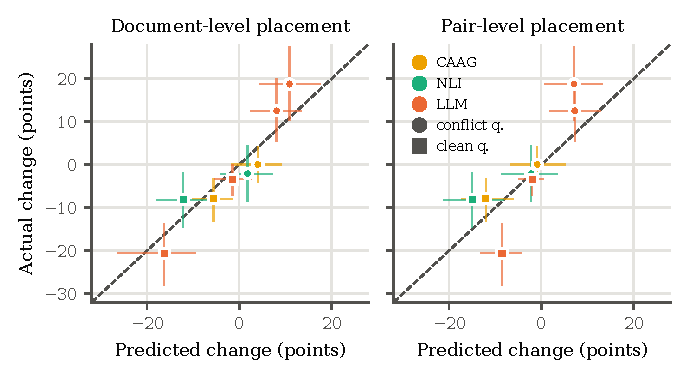
\includegraphics[width=\columnwidth]{generated/fig_placement.pdf}
\caption{Effect of real detectors predicted from the synthetic grid (x, with the 95\% bootstrap prediction interval)
against the measured effect (y, with its 95\% CI), for conflict ($\bullet$) and clean ($\blacksquare$) questions.
Left: detectors located by document-level behaviour; right: by pair precision, recall and direction accuracy.}
\label{fig:placement}
\end{figure}

\paragraph{The heuristic detector.}
CAAG, the detector we set out to study, scores a pair only if its MiniLM \citep{reimers2019sbert} cosine similarity reaches $\theta_s=0.65$. Its score
is the sum of a negation and contrast asymmetry term, a named-entity mismatch term (differing dates, numbers, money or
percentages) and a temporal-marker term, multiplied by the similarity; a pair is flagged at
$\theta_c=0.35$. Its per-pair flag rate on the confirmatory split ($6.22\%$) sets the random detector's rate.
As a neutral flag, CAAG did not beat random flags of the same volume, and
as a removal rule it only deleted correct passages (\dCaagRemClean\ points on clean questions, \dCaagRemConf\ on
conflict ones). Its false flags mostly hit pairs that should both be reported: 134 of 221 on the
hold-out are same-name ambiguity pairs, flagged by its entity-mismatch signal for differing dates or
numbers. We read this as a warning about lexical contradiction cues generally \citep{gururangan2018annotation},
not a particular threshold. Retuning shows why F1 misleads: over a 121-setting sweep, CAAG's
best pair F1 is \caagBestFOne, above NLI's, at $\theta_s=\caagBestThS$ and $\theta_c=\caagBestThC$, but it flags \caagBestRate\% of all pairs and \caagBestCleanFpr\% of clean questions, which our grid predicts
is harmful under removal (Appendix~\ref{app:grid}).

\paragraph{Original CAAG format.}
CAAG's flags in their original format, with typed lines and confidence scores (``factual conflict (confidence:
0.41)''), change accuracy by \origCaagAll\ points overall (\origCaagConf\ on conflict questions, \origCaagClean\ on
clean ones), no different from the uniform format.

\paragraph{Pilot study (exploratory).}
Before any confirmatory run, the 200-question pilot split, scored with the bidirectional metric, showed the same
pattern: oracle neutral flags changed conflict-question accuracy by $-$10.5 points, directional flags by
$+$11.8, and removing the suspect by $+$28.4. The pilots also showed that the original \textsc{remove} strategy,
which deletes an arbitrary side of each pair, removes correct documents, and led us to add directional formats,
synthetic direction accuracy and document-level placement. All pilot runs are released.

\paragraph{Phase-0 audit of CAAG on NarrativeQA.}
CAAG was designed for long-document QA. On 100 NarrativeQA \citep{kocisky2018narrativeqa} questions from 50 stories
(BM25 top-10 chunks from a single coherent story), it flags at least one pair in 54\% of questions, 166 pairs in all.
A single story rarely contradicts itself, so most flags are likely false. The flagged pairs are released for annotation.
